\documentclass{article}

\PassOptionsToPackage{super,sort&compress}{natbib}
\usepackage[dblblindworkshop]{neurips_2025}

% Standard packages
\usepackage{adjustbox}
\usepackage[utf8]{inputenc}
\usepackage[T1]{fontenc}
\usepackage{hyperref}
\usepackage{url}
\usepackage{booktabs}
\usepackage{amsfonts}
\usepackage{amsmath}
\usepackage{amssymb}
\usepackage{nicefrac}
\usepackage{microtype}
\usepackage{xcolor}
\usepackage{graphicx}
\usepackage[font=small,labelfont=bf]{caption}
\usepackage{subcaption}
\usepackage{threeparttable}
\usepackage{algorithm}
\usepackage{algorithmicx}
\usepackage{algpseudocode}
\usepackage{array}
\usepackage{svg}
\usepackage{enumitem}

\setcitestyle{super,comma,sort&compress}

\definecolor{cb_red}{HTML}{990000}
\definecolor{cb_green}{HTML}{AAFF80}

\title{A pipeline for interpretable neural latent discovery}
\workshoptitle{Data on the Brain \& Mind}

\author{
  Jai Bhagat \\
  Sainsbury Wellcome Centre \\
  University College London \\
  \texttt{jkbhagatio@gmail.com} \\
  \And
  Anaya Pouget \\
  Sainsbury Wellcome Centre \\
  University College London \\
  \texttt{pouget.anaya@gmail.com} \\
  \And
  Sara Molas Medina \\
  University College London \\
  \texttt{saramolas18@gmail.com} \\
}

\begin{document}

\maketitle

\begin{abstract}
Mechanistic understanding of the brain requires identifying interpretable latents composed of large-scale neuronal computations. We introduce MINI, a comprehensive pipeline for discovering and evaluating interpretable representations from neural data. MINI is designed to be a flexible, user-friendly tool for neuroscientists, featuring a modular architecture that can be adapted to various data types and experimental paradigms. We demonstrate MINI's utility on both synthetic and real-world neurophysiological data, showing that it can successfully identify meaningful, interpretable features.
\end{abstract}

\section{Introduction}

A central goal of modern neuroscience is to understand how the brain processes information to generate behavior. A promising approach is to use latent variable models (LVMs) to identify low-dimensional, interpretable representations from high-dimensional neural data. However, existing methods often require extensive hyperparameter tuning, are not easily adaptable to different data types, and lack standardized evaluation metrics. To address these challenges, we developed MINI, a pipeline for interpretable neural latent discovery. MINI is a modular, user-friendly toolkit that streamlines the process of data preprocessing, model training, and latent evaluation.

\section{Methods: The MINI pipeline}

\begin{figure}[h]
    \centering
    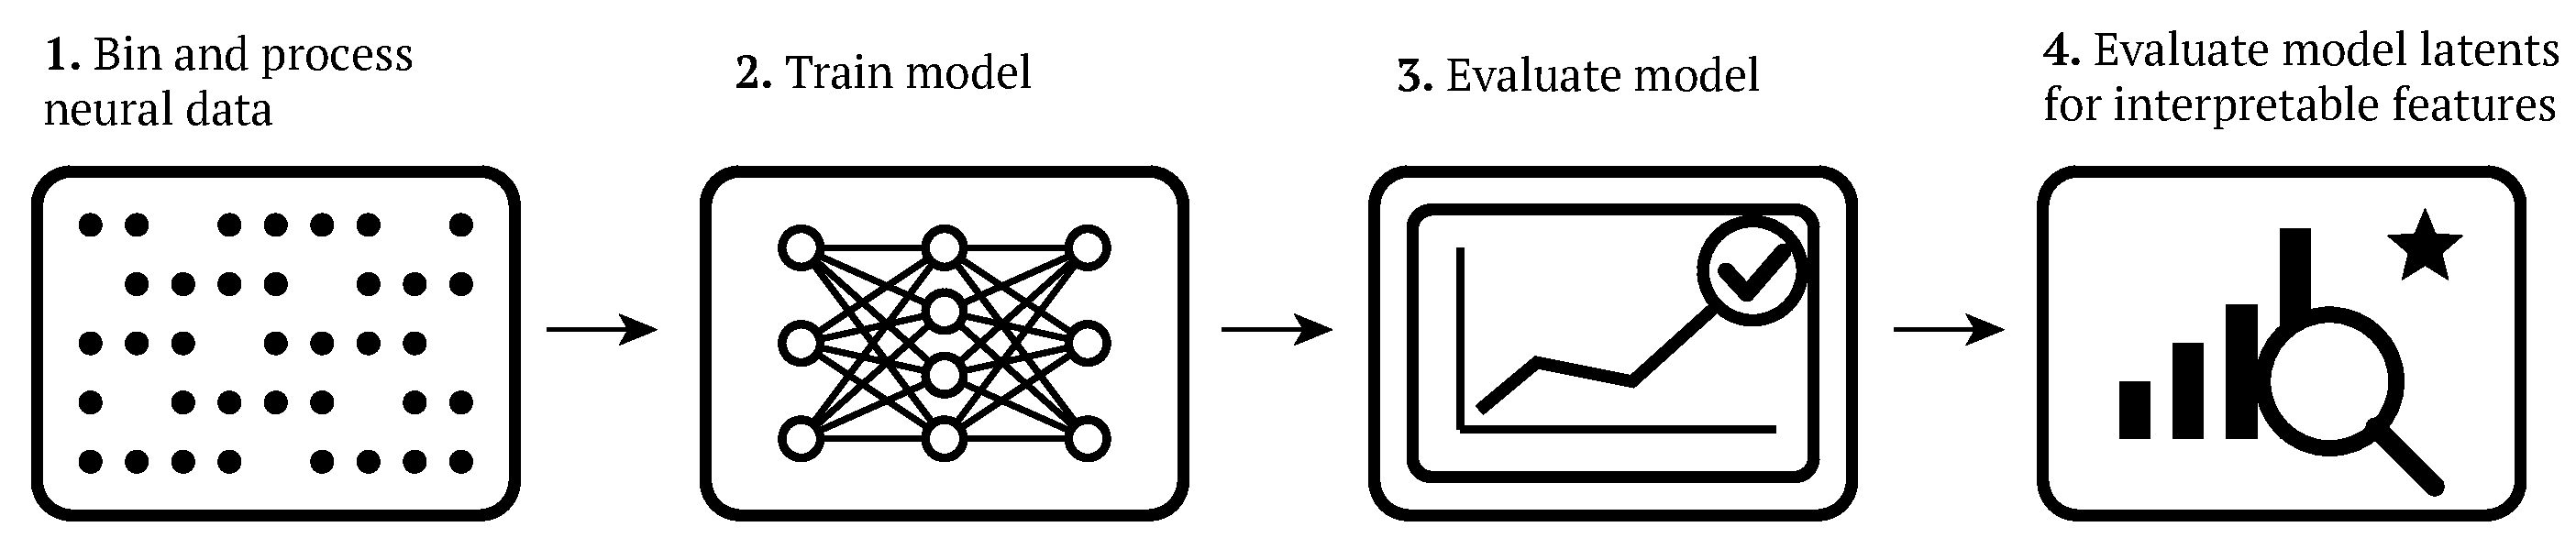
\includegraphics[width=\linewidth]{figures/mini_pipeline.pdf}
    \caption{
        \textbf{The MINI pipeline.} \\
        \small The MINI pipeline is comprised of 4 stages: 1) Spatiotemporal binning and processing of neural data; 2) Model training; 3) Model evaluation; 4) Latent evaluation for feature interpretability. Steps 1-3 can be either semi- or fully-automated.
    }
    \label{figure:mini_pipeline}
\end{figure}

The MINI pipeline transforms high-dimensional neural data into a set of interpretable latents in four primary stages (\autoref{figure:mini_pipeline}). The first stage prepares neural data for model training, including utilities for binning, and normalizing spike times. The second stage involves training a sparse dictionary neural network (SDNN) to reconstruct the neural data from a set of sparsely active dictionary elements. The model can be configured as an autoencoder, transcoder, or crosscoder. We use a Matryoshka architecture to learn a multi-scale feature representation, and batch top-k sparsity to enforce sparsity without a tunable regularization coefficient. An optional self-attention layer can be used to integrate information across time. The third and fourth stages involve model and latent evaluation, respectively.

\begin{figure}[htbp]
    \begin{minipage}{0.63\linewidth}
    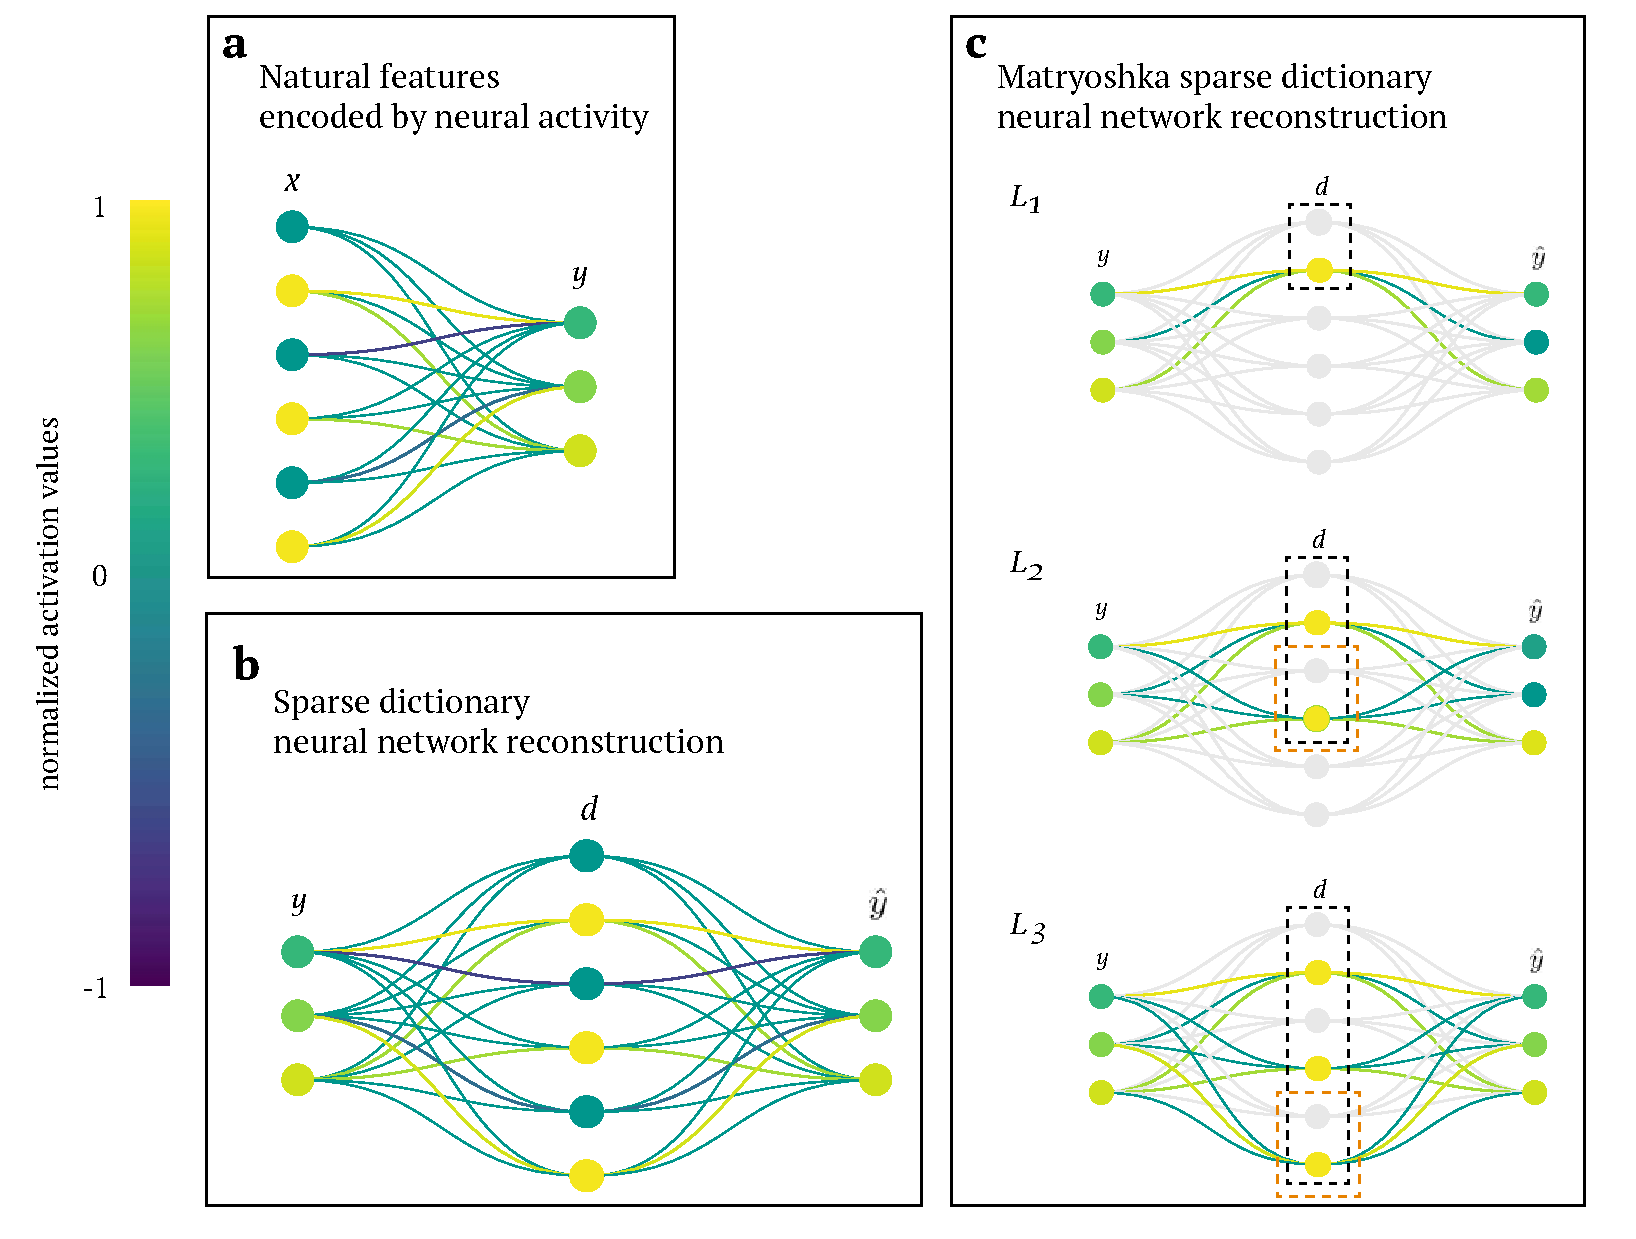
\includegraphics[width=\linewidth]{figures/sdnn_arch.pdf}
    \end{minipage}%
    \begin{minipage}{0.37\linewidth}
    \caption{
        \textbf{Model motivation} \\
        \small
        (\textbf{a}) Natural, "real-world" features $x$ are encoded by neural activity $y$. (\textbf{b}) A SDNN reconstructs neural activity $z$ based on $y$ via sparse dictionary elements $d$. When training is successful, $d$ corresponds to $x$. (\textbf{c}) A Matryoshka SDNN segments the latent space into multiple levels, each of which attempts a full reconstruction of the target neural activity, encouraging a multi-scale feature representation.
    }
    \label{figure:sdnn_arch}
    \end{minipage}
\end{figure}

\bibliographystyle{unsrt}
\bibliography{references}

\end{document}
